\documentclass{standalone}
% translate with >> pdflatex -shell-escape <file>

% This file is an extract of the PGFPLOTS manual, copyright by Christian Feuersaenger.
% 
% Feel free to use it as long as you cite the pgfplots manual properly.
%
% See
%   http://pgfplots.sourceforge.net/pgfplots.pdf
% for the complete manual.
%
% Any required input files (for <plot table> or <plot file> or the table package) can be downloaded
% at
% http://www.ctan.org/tex-archive/graphics/pgf/contrib/pgfplots/doc/latex/
% and
% http://www.ctan.org/tex-archive/graphics/pgf/contrib/pgfplots/doc/latex/plotdata/

\usepackage{pgfplots}
\pgfplotsset{compat=newest}

\pagestyle{empty}

\begin{document}
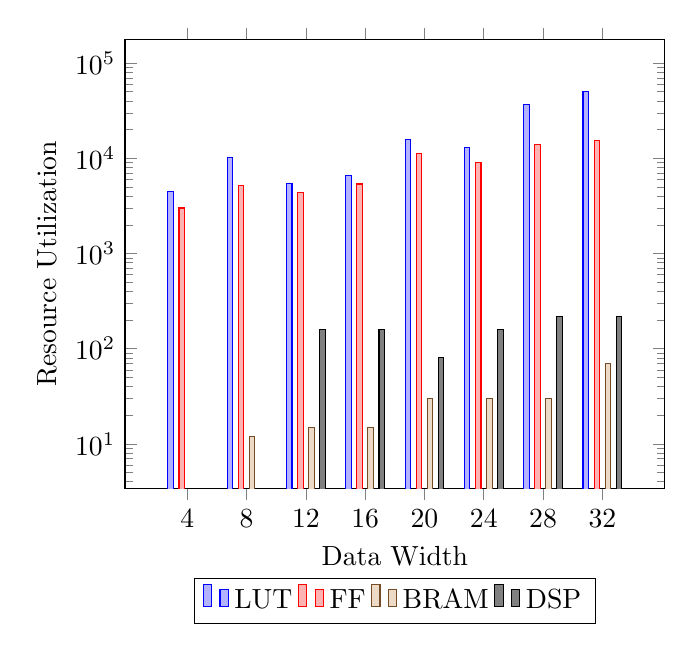
\begin{tikzpicture}
\begin{semilogyaxis}[
    ybar,
    enlargelimits=0.15,
    legend style={at={(0.5,-0.20)},
      anchor=north,legend columns=-1},
    ylabel={Resource Utilization},
    xlabel={Data Width},
    symbolic x coords={4,8,12,16,20,24,28,32},
    xtick=data,
    %nodes near coords,
    %nodes near coords align={horizontal},
    bar width=2pt,
    ]
\addplot coordinates {(4,4433) (8,10169) (12,5382) (16,6597) (20,15607) (24,13091) (28,36752) (32,50350)};
\addplot coordinates {(4,3007) (8,5166) (12,4364) (16,5368) (20,11147) (24,8966) (28,13931) (32,15544)};
\addplot coordinates {(4,0) (8,12) (12,15) (16,15) (20,30) (24,30) (28,30) (32,70)};
\addplot coordinates {(4,0) (8,0) (12,160) (16,160) (20,80) (24,160) (28,220) (32,220)};
\legend{LUT,FF,BRAM,DSP}
\end{semilogyaxis}
\end{tikzpicture}
\end{document}
